\documentclass[12pt]{article}
\usepackage{amsmath}
\usepackage{amssymb}
\usepackage{blindtext}
\usepackage{geometry}
\geometry{a5paper, margin=0.2in, bottom=0.5in}
\usepackage[english, russian]{babel}
\usepackage[utf8]{inputenc}
\usepackage{graphicx}
\usepackage{caption}
\usepackage{subcaption}
\usepackage{float}
\usepackage{comment}

\usepackage{listings}

\usepackage{indentfirst}

\graphicspath{ {./images/} }

\begin{document}

\section{Командная часть (Большие колебания)}

\subsection{Опыты}

Маятник:\\
g - ускорение свободного падения (\(g=9.81\text{ м/c}^2\)).\\
L - длина маятника (\(L=0.25\)м).\\
T - период.\\
M - момент силы (\(M=-mgL\sin{\theta}\)).\\
I - момент инерции (\(I=mL^2\)).\\
\(\omega\) - круговая частота колебаний (\(\omega=\sqrt{g/L}\approx6.26418\)).\\

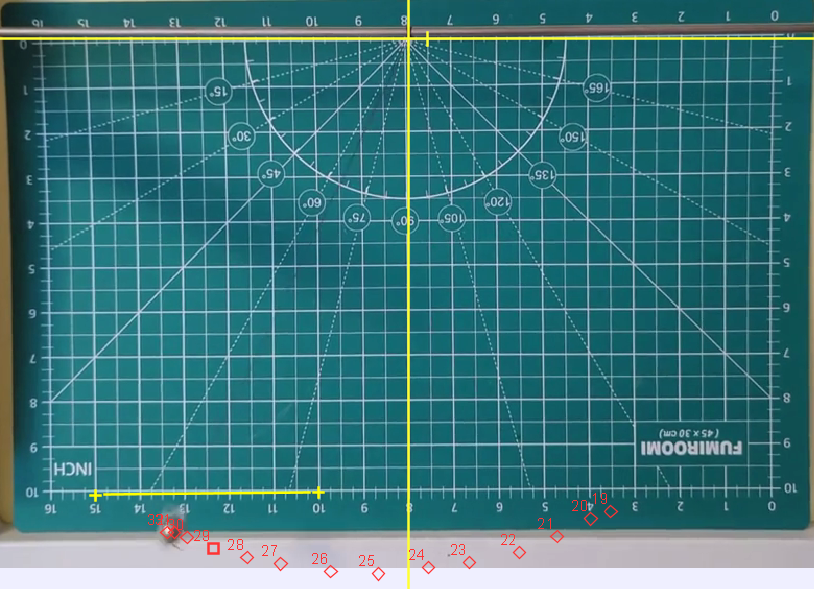
\includegraphics[width=0.75\linewidth]{pendulum.png}

\newpage

Опыт №1\\
\(\theta_0 = 20^\circ\) градусов.\\
Период \(T=1.00\).\\
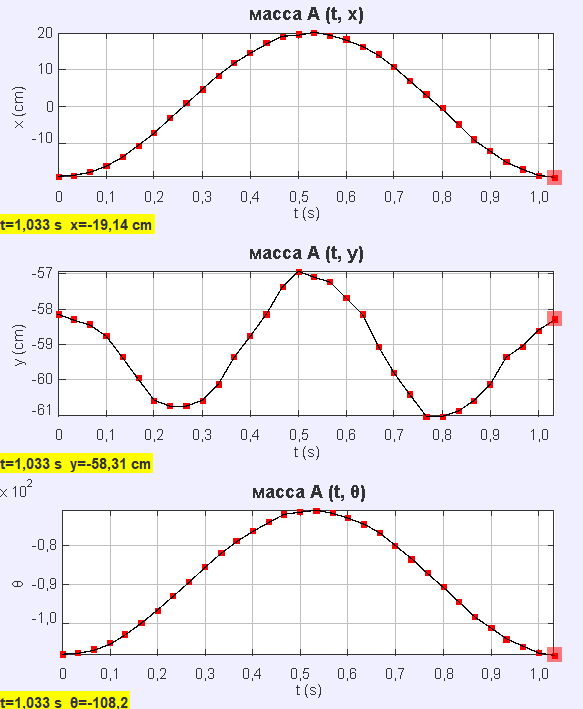
\includegraphics[width=0.6\linewidth]{graph20.png}

\newpage

Опыт №2\\
\(\theta_0 = 25^\circ\) градусов.\\
Период \(T=1.03\)с.\\
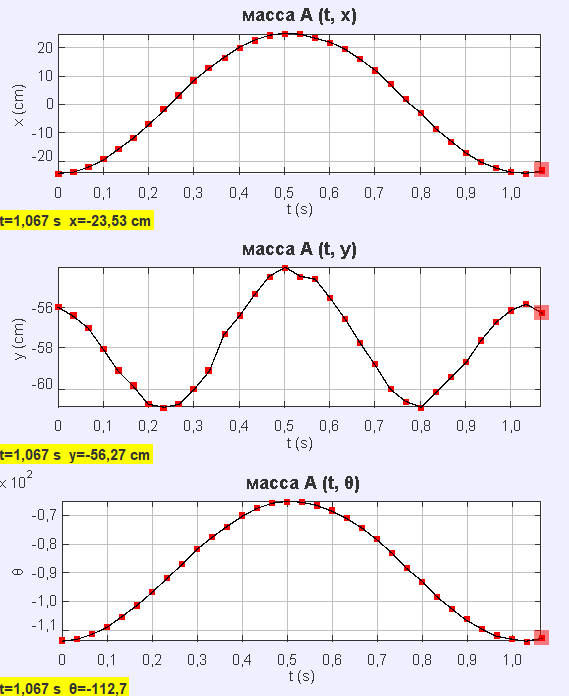
\includegraphics[width=0.6\linewidth]{graph25.png}

\newpage

Опыт №3\\
\(\theta_0 = 30^\circ\) градусов.\\
Период \(T=1.03\)с.\\
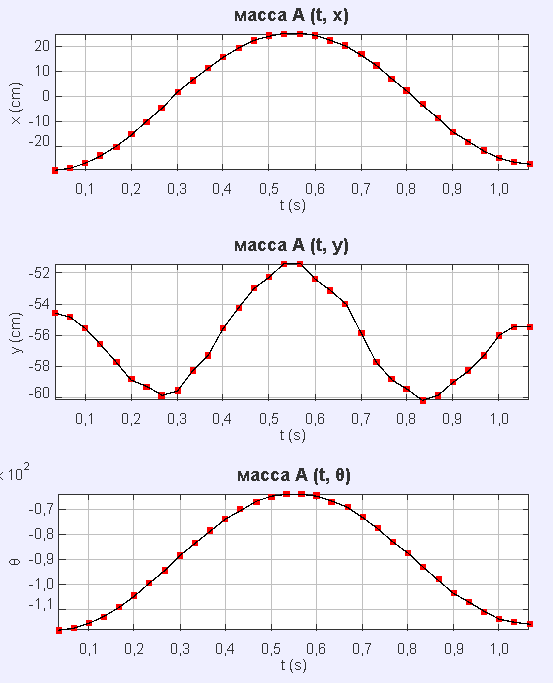
\includegraphics[width=0.6\linewidth]{graph30.png}

\newpage

\subsection{Отличие теории от практики}

формула (5)
\[T=\frac{2\sqrt{2}}{\omega}\int\limits_0^{\theta_0}{\frac{d\theta}{\sqrt{\cos{\theta}-\cos{\theta_0}}}}.\]

Главная загвоздка в комьютерном расчитывании этого интеграла в том, что выражение под корнем может равнятся нулю, то есть произойдет деление на 0. Чтобы такого не проиходило, мы как только можем уменьшим верхний предел и сделаем максимально мелкое разбиение.

Реализация такое программы на языке программирования python будет выглядеть примерно так:

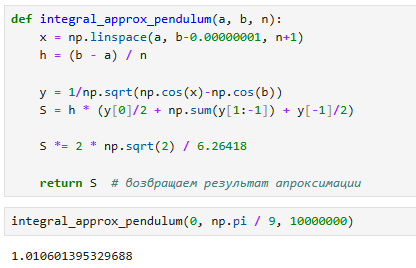
\includegraphics[width=0.6\linewidth]{pendulum_approx.png}

Опыт №1\\
\(T_{\text{прак}}=1.00\).\\
\(T_{\text{теор}}=\frac{2\sqrt{2}}{6.26418}\int\limits_0^{\pi/9}{\frac{d\theta}{\sqrt{\cos{\theta}-0.939692}}}=1.0106\)\\

Опыт №2\\
\(T_{\text{прак}}=1.03\).\\
\(T_{\text{теор}}=\frac{2\sqrt{2}}{6.26418}\int\limits_0^{\pi/7.2}{\frac{d\theta}{\sqrt{\cos{\theta}-0.906307}}}=1.0150\)\\

Опыт №3\\
\(T_{\text{прак}}=1.03\).\\
\(T_{\text{теор}}=\frac{2\sqrt{2}}{6.26418}\int\limits_0^{\pi/6}{\frac{d\theta}{\sqrt{\cos{\theta}-0.866025}}}=1.020415\)\\

\newpage

\subsection{Доказательство (6)}

\newpage

\subsection{Эллиптический интеграл}

\[K(k)=\int\limits_0^{\pi/2}\frac{du}{\sqrt{1-k^2\sin^2{u}}}=
\frac{\pi}{2}\sum\limits_{n=0}^{\infty}\left(\frac{(2n-1)!!}{(2n)!!}k^n\right)^2\]

Для \(n=0\):\\
\(\left(\frac{(2n-1)!!}{(2n)!!}k^n\right)^2=\left(\frac{(-1)!!}{(0)!!}\right)^2=1^2=1\)\\

Для \(n=1\):\\
\(\left(\frac{(2n-1)!!}{(2n)!!}k^n\right)^2=
\left(\frac{(1)!!}{(2)!!}k\right)^2=\left(\frac{1}{2}k\right)^2=\frac{k^2}{4}\)\\

Для \(n=2\):\\
\(\left(\frac{(2n-1)!!}{(2n)!!}k^n\right)^2=
\left(\frac{(3)!!}{(4)!!}k^2\right)^2=
\left(\frac{1 \cdot 3}{2 \cdot 4}k^2\right)^2=\frac{9k^4}{64}\)\\

Значит при \(n=2\):\\
\[K(k)=\frac{\pi}{2}\left(1+\frac{k^2}{4}+\frac{9k^4}{64}\right)\]
    
\newpage

Полный эллиптический интеграл первого рода может использоваться для расчетов периода колебаний математического маятника с большой амплитудой. Например по вот такой формуле:

\[T=\frac{4}{\omega _{0}}K\left(\sin \frac{\theta _{0}}{2}\right)\]

Рассмотрим \(\theta_0 = 30^{\circ}, \sin{\frac{\theta_0}{2}=0.2588}\) для примера с нашим маятником. Тогда 

При \(n=0\):\\
\(T=\frac{4}{6.26418}K\left(\sin \frac{\theta_{0}}{2}\right)=
0.638551 \cdot \frac{\pi}{2}=1.00302\)\\

При \(n=1\):\\
\(T=\frac{4}{6.26418}K\left(\sin \frac{\theta_{0}}{2}\right)=
0.638551 \cdot \frac{\pi}{2}(1+\frac{\sin^2{\frac{\theta_0}{2}}}{4})=
1.00302 \cdot (1+\frac{0.2588^2}{4})=1.00302 \cdot 1.016746 = 1.0198165\)\\

При \(n=2\):\\
\(T=\frac{4}{6.26418}K\left(\sin \frac{\theta_{0}}{2}\right)=
0.638551 \cdot \frac{\pi}{2}(1+\frac{\sin^2{(15^\circ)}}{4}+\frac{9\sin^4{(15^\circ)}}{64})=
1.00302 \cdot (1+\frac{0.2588^2}{4}+\frac{0.2588^4}{64})=
1.00302 \cdot (1 + 0.016746 + 0.000070) = 1.0198868\)\\

\newpage

\subsection{Оценка погрешностей и выводы}
 Во время проведения эксперимента источником погрешности были:
\begin{itemize}
  \item Неточность измерения длины L.
  \item Неточность определения угла \(\theta_0\).
  \item Сопротивление воздуха, трение в подвесе.
  \item Малая частота кадров, плохое качество видео.
\end{itemize}
А во время вычислений:
\begin{itemize}
  \item Погрешность компьютерных вычислений.
  \item Погрешность от использования конечного числа членов ряда (7).
\end{itemize}
\textbf{Выводы}:

Нелинейная модель точнее описывает движение при больших амплитудах.

Ряд (7) позволяет удобно вычислять период без численного интегрирования, но при больших углах требует многих членов.

\end{document}

